% !TEX root = ./main.tex
\section{Preliminaries}
\label{sec:background}
\begin{figure}
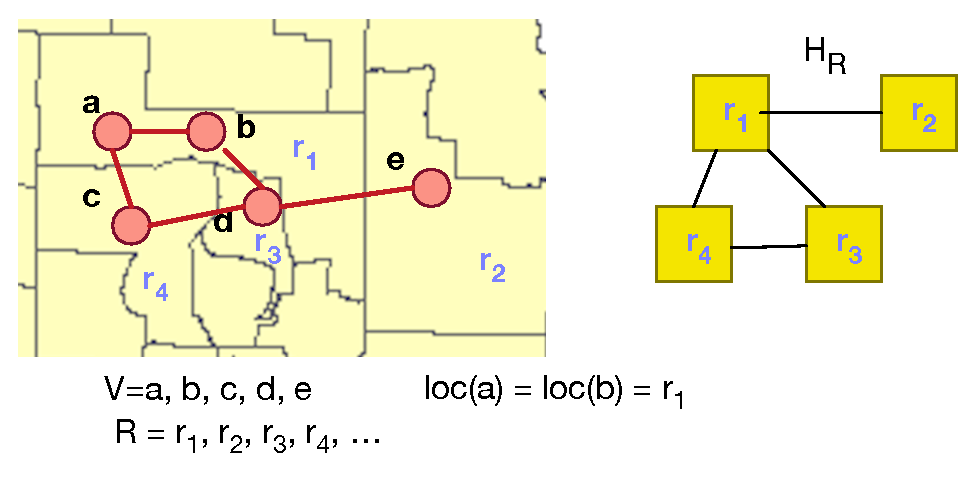
\includegraphics[width=0.45\textwidth]{img/example.pdf}
\vspace{-.2in}
\caption{Notation used in the paper. The 5 red circle nodes $(a,b,c,d,e)$ form a social contact network. Each node resides in a block group $r_i$, and these block groups form the block group graph $H_\mathcal{R}$, where an edge represents that the block groups are adjacent on the map.}
\label{fig:definitions-example}
\end{figure}
\subsection{Disease spread on a social contact network}
Let $V$ denote a population, and let $G=(V, E)$ be a contact graph on which a disease can spread. A person or node $v \in V$ can propagate the disease to its neighbors. There is an edge between two people if they come into close proximity during a typical day. For example, the nodes represent two coworkers in the same building, students in the same classroom, or members of the same household. 
Additionally, %in the social contact network datasets that we consider (Section \ref{sec:data}),
each person $v$ is associated with a geographical location---i.e., their place of residence---denoted by $\loc(v)$;
we will consider such locations at the resolution of census block groups.
Let $\mathcal{R}$ denote the geographical area where the nodes $V$ are located---for example, the state of Minnesota---and let $\mathcal{R}=\{r_1,\ldots,r_N\}$ be a decomposition of $\mathcal{R}$ into
census block groups. For a block group $r_i\in\mathcal{R}$, we use $V(r_i)$ to denote the
set of nodes associated with location $r_i$; that is, those with $\loc(v)\in r_i$. Analogously, for a set of block groups or \emph{region} $R\subset \R$, let $V(R)=\cup_{r_i\in R} V(r_i)$ be the set of nodes located within $R$. We consider a graph $H_{\R}=(\R, E_{\R})$ on the set of block groups, where
two block groups are connected if they are geographically contiguous, i.e., they are adjacent on a map. In particular, we are interested in \emph{connected} subgraphs of $H_{\R}$. We use $\ConnR$ to denote all the subsets $R\subset \HR$ that are spatially connected. These definitions are illustrated in Figure \ref{fig:definitions-example}.
%$(R_i, R_j)\in E_{\R}$ if $R_i$ and $R_j$ have a common boundary.
%Let $\ConnR$ denote subsets $R\subset \HR$ that are spatially connected in the block group graph $H_{\R}$.

\begin{table}[ht]
\begin{footnotesize}
\centering \caption{
Summary of the notation used in the paper
}
\label{table:notation}
\begin{tabular}{|p{0.9in}|p{2.2in}|}
\hline
\textbf{Notation} & \textbf{Description} \\
\hline
$G=(V, E)$ & Contact graph on set $V$ of individuals\\
$\loc(v)$ & Geographical location of node $v$\\
$\mathcal{R}=\{r_1,\ldots,r_N\}$ & Entire geographical area where the nodes $V$ are located---e.g., Minnesota partitioned into block groups $r_i$\\
$V(r_i)$ & Set of nodes of $G$ with $\loc(v)=r_i$\\
$V(R)$ & $\cup_{r_i\in R} V(r_i)$\\
$H_{\R}=(\R, E_{\R})$ & Network on $\R$, with adjacent block groups connected by an edge.
Sometimes referred to as ``the auxiliary network.''\\
$\ConnR$ & Set $R\subset \R$  spatially connected in $H_{\R}$\\
%S, E, I, R & States in the disease model\\
$\gamma$ & Average region-wide vaccination rate\\
$\mathbf{x}$ & Vaccination vector, with $x_i$ denoting the probability that node $i$
is vaccinated\\
$\mathbf{x}^R$ & Vaccination vector, with nodes $V(R)$ undervaccinated, where $R\in\ConnR$\\
$\src_A$, $\src$ & Denotes the event that the  infection source is from a 
set $A\subset \R$. $\src$ is used when $A=\R$ \\
$\numinf(\mathbf{x}, \src_A)$ & Expected number of infections for
vaccination vector $\mathbf{x}$ and source being $\src_A$\\
%$\crit(R, \mathbf{x}, \src_A)$ & Criticality of $R$: expected number of additional infections if $R$ is not vaccinated\\
$\maxcrit(R)$, $\maxcrit(R, \mathbf{x})$ & The objective value of $\maxcrit{}$ for region
$R\in\ConnR$ in an instance $(G, H_{\R}, k)$\\
%$\avgcrit(R)$, $\avgcrit(R, \mathbf{x})$ & The objective value of $\avgcrit{}$ for region
%$R\in\ConnR$ in an instance $(G, H_{\R}, k)$\\
\hline
\end{tabular}
\end{footnotesize}
\end{table}

\noindent
\textbf{Distances and geometry of $\HR$.}
For $u, v\in \R$, let $\dist_{\HR}(u, v)$ denote the distance between $u$ and $v$ in the graph $\HR$, which is equal to the length of the shortest path between them.
The ball centered at $v$, with radius $\ell$ is defined as $B_{\HR}(v, \ell)=\{u: \dist(u, v)\leq\ell\}$, which is the set of all nodes within distance $\ell$ of $v$. When the graph is clear from the context, we drop it from the subscript in the notation for $B(\cdot)$ and $\dist(\cdot)$.
We say that the graph $\HR$ has \emph{doubling dimension} $d$ if it satisfies the following property: any ball $B(v, \ell)$ can be covered by at most $2^d$ balls of radius $\ell/2$ \cite{gupta:focs03}. Geometric graphs, such as grids, have constant doubling dimension, usually around $2$; note that $d$ need not be an integer. Our approximation guarantees will be in terms of $d$.

\noindent
\textbf{Disease model.} We use an SEIR model for diseases like measles \cite{anderson+m:book}, 
where a node is in one of four states:
Susceptible (S), Exposed (E), Infected (I), and Recovered/Removed (R). Measles is highly contagious, and an infected node spreads the
disease to each susceptible neighbor with high probability. 
Sometimes, we assume a transmission probability of 1, but our results
extend to the more general case. If a node is vaccinated,
it does not get infected. We assume the vaccine has 100\% efficacy, which is
not true in practice, but this is not crucial for our methodology.

Let $\gamma$ denote the average region-wide vaccination rate---around $0.97$
in Minnesota. Let $\mathbf{x}$ be a \emph{vaccination} or \emph{intervention} vector: 
$x_i\in[0,1]$ denotes the probability that node $i$ is vaccinated (so $x_i=\gamma$,
by default).
Let $\src_A$ denote the source of the infection or \emph{initial conditions} of the disease process: this could be one or a small number of nodes from a region $A\subset \mathcal{R}$, which initially get infected. We use $\numinf(\mathbf{x}, \src_A)$ to denote the expected number of infections
given an intervention $\mathbf{x}$ and initial conditions $\src_A$.
When $\src_A$ is clear from the context, we simply use $\numinf(\mathbf{x})$.
  
%\subsection{Criticality and Problem Formulation}
\subsection{Criticality}
For a vaccination vector $\mathbf{x}$,
let $\mathbf{x}^S$ denote the corresponding intervention where a subset $S\subset V$ of
nodes is undervaccinated. That is,
$\mathbf{x}^S_i = \mathbf{x}_i$ for $i\not\in S$ and $\mathbf{x}^S_i=\gamma'$ for $i\in S$,
where $\gamma'$ is much lower than $\gamma$, the region-wide vaccination rate.
Without loss of generality, we sometimes consider $\gamma'=0$ for mathematical convenience.

\setlength{\abovedisplayskip}{3pt}
\setlength{\belowdisplayskip}{3pt}

%We define the \textbf{criticality} of a set $S\subset V$ as
%$\crit(S, \mathbf{x}, \src_A) = \numinf(\mathbf{x}^S, \src_A) - \numinf(\mathbf{x}, \src_A)$,
%which is the \emph{expected number of additional infections that occur if $S$ is not vaccinated}
%(with respect to any specific initial conditions $\src_A$).
%Our focus is on finding spatial clusters of high criticality, so %Therefore, the set $S$
%of nodes in the above notion of criticality must be located in a connected geographical region.
%we focus on $S=V(R)$ for a connected region $R\in\ConnR$.

We define the \textbf{criticality} of a set $S\subset V$ as
the \emph{expected number of additional infections that occur if $S$ is not vaccinated},
with respect to some initial condition $\src_A$.
Because we are interested on finding spatial clusters of high criticality, 
we focus on $S=V(R)$ for a connected region $R\in\ConnR$.
Then, we define the criticality of a region as
\[
\crit(R, \mathbf{x}, \src_A) = \numinf(\mathbf{x}^R, \src_A) - \numinf(\mathbf{x}, \src_A),
\]
which is the expected number of extra infections if nodes in the region $R$ are undervaccinated. In order to simplify the notation, we will drop $\mathbf{x}$ and $\src$ from the inputs to $\crit(\cdot)$, whenever it is clear from the context.


%Then, we pose the task of finding spatial clusters of high criticality as the following optimization problem.

\section{Problem Formulation}
\label{sec:problem-statement}

\noindent 
\textbf{Modeling considerations.} In practice, public health interventions involve intensive field work---e.g., targeted information campaigns. Furthermore, these interventions are most effective within small, localized geographical regions. Therefore, we focus on finding regions that have high criticality \emph{and} small size. In modeling terms, this can be accomplished by adding a size parameter $k$, which can be tuned based on the available public health resources. 

Given the discussion above, we pose the task of finding spatial clusters of high criticality as the following optimization problem.
\begin{problem}[$\maxcrit{}(G, H_{\R}, k)$]
\label{prob:maxcrit}
Given an instance $(G, H_{\R}, k)$, find a connected region $R\in\ConnR$ of size at most $k$ that maximizes criticality over all choices of source:
\[
R= \mbox{\emph{argmax}}_{R'\in\ConnR, |R'|\leq k} \text{\emph{crit}}(R', \mathbf{x}, \src_{R'})
\]
\end{problem}

In words, the $\maxcrit{}$ problem involves maximizing over \emph{all} possible
choices of the sources $\src_{R'}$ in the cluster $R'$. We emphasize that the disease spreads on the social network $G$ of \emph{individuals}, whereas the connectivity constraint is imposed on the graph $\HR$ of \emph{census block groups}, since we're interested in finding a spatial cluster. From a public health perspective, our problem models the following question: \emph{what is the most critical cluster of size $k$ if the disease starts within the undervaccinated cluster itself?} An obvious question is how should the parameter $k$ be chosen. As mentioned earlier, this can depend on the resources of the public health department, since interventions are very localized.

% This is formalized as
%We use $\maxcrit(R, \mathbf{x}, \src)$ or 
%$\maxcrit(R)$ to denote the objective value of an instance of the problem.


% $\max_{\src_R} \crit(R, \mathbf{x}, \src_R)$, the objective value of $\maxcrit{}$ for region $R$ in an instance $(G, H_{\R}, k)$.



%\subsection{Submodularity}
%A set function $f: 2^V \rightarrow \mathbb{R}$ is said to be \emph{submodular} if it satisfies the diminishing returns property: for any $T \subset S\subset V$ and $x \in V\setminus S$, we have that
%$$
%f(T \cup x) - f(T) \geq f(S \cup x) - f(S).
%$$
%That is, the marginal gain of adding $x$ to a set is larger on a smaller context. 
%
%Submodularity has become popular in recent years in machine learning \cite{krause2008beyond} because 1) the diminishing returns property applies naturally to many problems of interest (e.g., sensor placement) and 2) there exist simple algorithms for approximate constrained submodularity maximization \cite{nemhauser1978analysis}---though the problem is NP-Hard in general. For the problem of maximizing a submodular function over subsets of size at most $k$, Nemhauser et al.\ \cite{nemhauser1978analysis} proposes the following greedy algorithm. We start with the empty set $S_0 = \emptyset$. We construct a set $S_i$ by adding an element to $S_{i-1}$ that yields the highest increase in objective value:
%$$
%S_{i} = S_{i - 1} \cup \operatornamewithlimits{argmax}_{x \in V \setminus S_{i - 1}} \{f(S_{i - 1} \cup \{x\}) - f(S_{i - 1})\}
%$$
%The algorithm returns a set $S_k$ as the solution, with objective value at least $1 - \frac{1}{e}$ of the optimal. We refer to this procedure as \emph{the greedy algorithm}.
%
%We focus on submodular function maximization with connectivity constraints.
%\begin{problem}
%\label{prob:connected-submodular}
%Given a graph $G=(V,E)$, a non-negative submodular function $f: 2^V \rightarrow \mathbb{R}^+$, and a parameter $k$, the objective is to find a set $S\subset V$ of size at most $k$ that maximizes $f$.
%\end{problem}
%
%As we discuss in Section \ref{sec:proposed-critical}, the \kcsp{} and \kcrp{} problems are equivalent to Problem \ref{prob:connected-submodular}.
%
%
%\subsection{Notes on problem formulations}
%
%Extending the earlier definitions to take initial conditions into account.
%\begin{itemize}
%\item
%Let $\mathbf{s}$ be a distribution specifying the source. 
%\item
%Let $Src_A$ denote the event that the source is in set $A$ of block groups. Let
%$p(Src_A)$ denote the probability of this event; it is proportional to the number of
%block groups in $A$
%\item
%$\numinf(\mathbf{x}, \mathbf{s})$ is the expected number of infections that occur
%when the intervention vector is $\mathbf{x}$ and the source is distributed according to
%the distribution $\mathbf{s}$. 
%\item
%$\numinf(\mathbf{x}, Src_A)$ is the expected number of infections that occur, conditioned
%on the event $Src_A$ occurring, i.e., if the source is uniformly distributed in $A$
%\item
%$\avgcrit(S, \mathbf{x}, \mathbf{s}) = \numinf(\mathbf{x}^S, \mathbf{s}) - 
%\numinf(\mathbf{x}, \mathbf{s})$ is the criticality of $S$, 
%where $\mathbf{s}$ denotes a set of sources.
%\item
%$\maxcrit(S, \mathbf{x}) = \max_{\mathbf{s}} \numinf(\mathbf{x}^S, \mathbf{s}) - 
%\numinf(\mathbf{x}, \mathbf{s})$ is the criticality of $S$, over all possible source distributions.
%In practice, $\maxcrit(S)$ will be maximized for an event $Src_S$, i.e., when the source
%is actually in $S$.
%\item
%Problem 1: critical set when the source is distributed independently. 
%Given a set $\mathbf{s}$ of sources, this is formalized as the following problem
%\[
%\mbox{argmax}_{R', |R'|\leq k} \avgcrit(R', \mathbf{x}, \mathbf{s})
%\]
%\item
%Problem 2: critical set when the source is chosen to be one that maximizes the criticality.
%This is formalized as the following problem
%\[
%\mbox{argmax}_{|R'|\leq k} \maxcrit(R', \mathbf{x})
%\]
%\end{itemize}
%
%Some observations
%\begin{itemize}
%\item
%For any monotone function $F(\cdot)$ and disjoint sets $A_1, A_2$,
%we have $F(A_1\cup A_2) \geq \frac{1}{2}F(A_1) + \frac{1}{2}F(A_2)$. This follows from the
%following reason: suppose $F(A_1)\geq F(A_2)$. Then, by monotonicity, we have
%\[
%F(A_1\cup A_2)\geq F(A_1)\geq \frac{1}{2}F(A_1) + \frac{1}{2}F(A_1) \geq \frac{1}{2}F(A_1) + \frac{1}{2}F(A_2) 
%\]
%Such a property does not imply $(r, \gamma)$-locality in \cite{krause2006near}, because
%they need the following property: for disjoint sets $A_1, A_2,\ldots, A_k$
%\[
%F(A_1\cup A_2\cup\ldots A_k)\geq \gamma\sum_{i=1}^k F(A_i)
%\]
%If the stronger property of $(r, \gamma)$-locality from \cite{krause2006near} holds, then
%the above property follows because
%\begin{eqnarray*}
%F(A_1\cup A_2\cup\ldots A_k) &\geq& F(A_1\cup A_2\cup\ldots A_{k-1}) + \gamma F(A_k)\\
%&\geq& F(A_1\cup A_2\cup\ldots A_{k-2}) + \gamma F(A_{k-1}) + \gamma F(A_k)\\
%&\geq& \ldots
%\end{eqnarray*}
%\item
%The objective $\maxcrit(\cdot)$ is not $(r,\gamma)$ local. Consider a setting
%where each block group induces a clique, which is disjoint from all other block groups.
%Then, $\maxcrit(A_1)\propto \max_{b\in A_1} |V(b)|$ is proportional to the largest
%block group in the set $A_1$. Similarly, we have $\maxcrit(A_2)\propto \max_{b\in A_2} |V(b)|$.
%For disjoint sets $A_1, A_2$, we have
%\[
%\maxcrit(A_1\cup A_2) = \max_{b\in A_1\cup A_2} |V(b)| < \maxcrit(A_1) + \maxcrit(A_2)
%\]
%\item
%The solutions are different for these formulations can be different. 
%Suppose a graph has is a large 
%Solutions that optimize
%$\maxcrit(\cdot)$ will be large clusters, which are s
%\end{itemize}
%
%\comment{somewhere: put justification for both problems and using synthetic populations}

